\let\negmedspace\undefined
\let\negthickspace\undefined
\documentclass[journal]{IEEEtran}
\usepackage[a5paper, margin=10mm, onecolumn]{geometry}
%\usepackage{lmodern} % Ensure lmodern is loaded for pdflatex
\usepackage{tfrupee} % Include tfrupee package

\setlength{\headheight}{1cm} % Set the height of the header box
\setlength{\headsep}{0mm}     % Set the distance between the header box and the top of the text

\usepackage{gvv-book}
\usepackage{gvv}
\usepackage{cite}
\usepackage{amsmath,amssymb,amsfonts,amsthm}
\usepackage{algorithmic}
\usepackage{graphicx}
\usepackage{textcomp}
\usepackage{xcolor}
\usepackage{txfonts}
\usepackage{listings}
\usepackage{enumitem}
\usepackage{mathtools}
\usepackage{gensymb}
\usepackage{comment}
\usepackage[breaklinks=true]{hyperref}
\usepackage{tkz-euclide} 
\usepackage{listings}
% \usepackage{gvv}                                        
\def\inputGnumericTable{}                                 
\usepackage[latin1]{inputenc}                                
\usepackage{color}                                            
\usepackage{array}                                            
\usepackage{longtable}                                       
\usepackage{calc}                                             
\usepackage{multirow}                                         
\usepackage{hhline}                                           
\usepackage{ifthen}                                           
\usepackage{lscape}
\usetikzlibrary{angles, quotes}
\begin{document}

\bibliographystyle{IEEEtran}
\vspace{3cm}

\title{12.8.3.5}
\author{EE24BTECH11055 - Sai Akhila Reddy Turpu}
% \maketitle
% \newpage
% \bigskip
{\let\newpage\relax\maketitle}

\renewcommand{\thefigure}{\theenumi}
\renewcommand{\thetable}{\theenumi}
\setlength{\intextsep}{10pt} % Space between text and floats


\numberwithin{equation}{enumi}
\numberwithin{figure}{enumi}
\renewcommand{\thetable}{\theenumi}

% Question
\section*{Question:}
\begin{align}
\text{Find the area bounded by the curve } y=\sin{x} \text{ between } x=0 \text{ and } x=2\pi
\end{align}
%  Solution
\section*{Using Trapezoidal rule to solve the given Integration problem: }
The trapezoidal rule is a numerical method for approximating the definite integral of a function. It works by dividing the area under the curve into trapezoids and summing their areas to estimate the total integral.\\\\
THE BASIC TRAPEZOIDAL RULE:\\
The trapezoidal rule is a numerical method for approximating the definite integral of a function. It works by dividing the area under the curve into trapezoids and summing their areas to estimate the total integral. The method is particularly useful when the exact integral is difficult or impossible to compute analytically.\\
Definition:\\
Let f\brak{x} be a continuous function defined on the interval \sbrak{a,b}. The definite integral $\int_a^bf(x)\,dx$ can be approximated using the trapezoidal rule as:\\
\begin{align}
\int_a^bf(x)\,dx\approx\frac{b-a}{2}\sbrak{f\brak{a}+f\brak{b}}
\end{align}
TRAPEZOIDAL RULE WITH SUB-INTERVALS:\\
If we divide $\sbrak{a,b}$ into $n$ sub-intervals of equal width $h=\frac{b-a}{n}$ then the approximation becomes more accurate. The interval $\sbrak{a,b}$ is divided into points:\\
\begin{align}
    x_0=a,x_1=a+h,x_2=a+2h,.....,x_n=b
\end{align}
The trapezoidal rule for $n$ sub-intervals is:(The sum of areas of all sub-trapezoids within the curve)\\
\begin{align}
    \int_a^bf(x)\,dx\approx \frac{h}{2}\sbrak{f\brak{x_0}+2f\brak{x_1}+.....+2f\brak{x_{n-1}}+f\brak{x_n}}
\end{align}
Or equivalently:\\
\begin{align}
    \int_a^bf(x)\,dx\approx \frac{h}{2}\sbrak{f\brak{a}+2\sum_{i=1}^{n-1}f\brak{x_i}+f\brak{b}}
\end{align}
Taking trapezoids of small width of h discretising points on the $x$ axis $x_0, x_1, x_2, \dots, x_n$.The sum of the trapezoidal areas will be
\begin{align}
    A&=\frac{1}{2}h\brak{y\brak{x_1}+y\brak{x_0}}+ \frac{1}{2}h\brak{y\brak{x_2}+y\brak{x_1}}+\dots+\frac{1}{2}h\brak{y\brak{x_n}+y\brak{x_{n-1}}}\\
  &=h\sbrak{\frac{1}{2}\brak{y\brak{x_0}+y\brak{x_n}}+ y\brak{x_1}+\dots+y\brak{x_{n-1}}}
\end{align}
Let $A\brak{x_n}$ be the area enclosed by the curve $y\brak{x}$ from $x=x_0$ to $x=x_n$, $\brak{x_0, x_1, \dots x_n}$ be equidistant points with step-size $h$.
\begin{align}
  A\brak{x_n+h}=A\brak{x_n}+\frac{1}{2}h\brak{y\brak{x_n+h}+y\brak{x_n}}
\end{align}
We repeat this until we get the required area.\\
Discretizing the steps, making $A\brak{x_n}=A_n, y\brak{x_n}=y_n$ we get,
\begin{align}
 A_{n+1}=A_n+\frac{1}{2}h\brak{y_{n+1}+y_n}
\end{align}
We can write $y_{n+1}$ in terms of $y_n$ using first principle of derivative. $y_{n+1}=y_n+hy^{\prime}_n$
\begin{align}
  A_{n+1}&=A_n+\frac{1}{2}h\brak{\brak{y_{n}+hy^{\prime}_n}+y_n}\\
  A_{n+1}&=A_n+\frac{1}{2}h\brak{2y_n+hy^{\prime}_n}\\
  A_{n+1}&=A_n+hy_n+\frac{1}{2}h^2y^{\prime}_n\\
  x_{n+1}&=x_n+h
\end{align}

In the given question, $y_n=\sin{(x_n)}$ and $y^{\prime}_n=\cos{(x_n)}$\\
General Difference Equation will be given by,
\begin{align}
  A_{n+1}&=A_n+hy_n+\frac{1}{2}h^2y^{\prime}_n\\
  &=A_n+h\brak{\sin{x_n}}+\frac{1}{2}h^2\brak{\cos{x_n}}\\
  x_{n+1}&=x_n+h
\end{align}
Iterating till we reach $x_n=\pi$ will return required area.\\
Area obtained computationally: $1.999988$ sq. units\\
Area obtained theoretically: $4$ sq. units.\\
As $n$ tends to infinity $A_n$ will be the exact area of the ellipse.

\begin{figure}[h!]
    \centering
    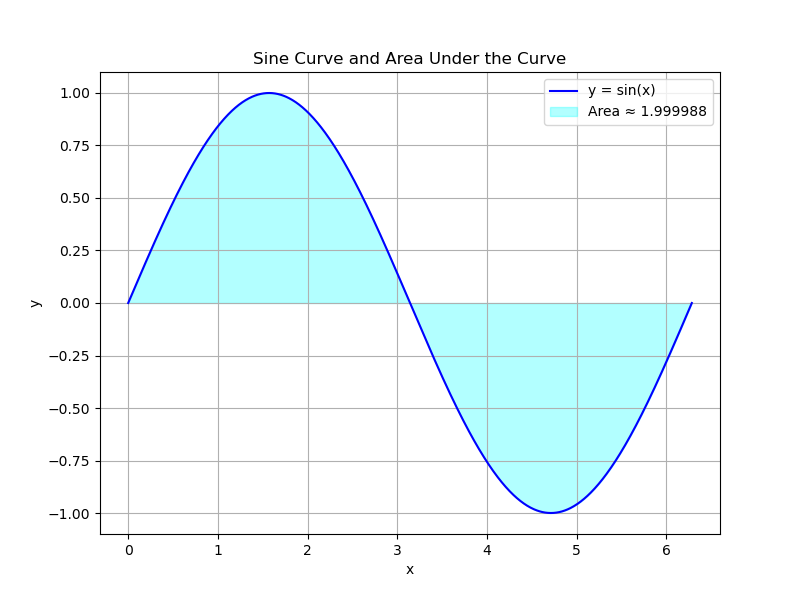
\includegraphics[width=\columnwidth]{figs/i.png}
    \caption{Sine Curve and Area Under the Curve}
    \label{fig:sine_curve}
\end{figure}


\end{document}
